\section{Expressing linear equations}
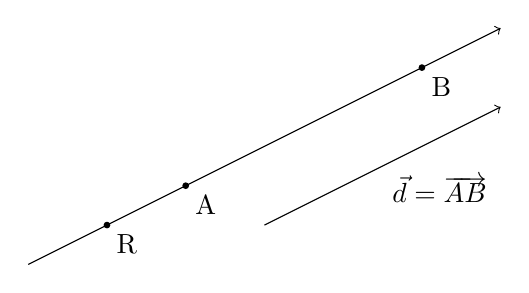
\begin{tikzpicture}
	\draw[->] (0,0) -- (6,3);
	\node[below right] at (1,0.5) {R};
	\filldraw [black] (1,0.5) circle (1pt);
	\node[below right] at (2,1) {A};
	\filldraw [black] (2,1) circle (1pt);
	\node[below right] at (5,2.5) {B};
	\filldraw [black] (5,2.5) circle (1pt);
	\draw[->] (3,0.5) -- (6,2);
	\node[below right] at (4.5,1.25) {$\vec{d}=\overrightarrow{AB}$};
\end{tikzpicture}

\subsection{Vector form}
$\vec{r}=\vec{a}+t\vec{d}$ or $(\vec{r}-\vec{a})\times\vec{d}=0$ / $(\vec{r}-\vec{a})\times\vec{b}=0$
\subsection{Parametric form}
$\begin{cases}
	x=x_0+tu\\
	y=y_0+tv\\
	z=z_0+tw
\end{cases}$
\subsection{Cartesian form}
$\dfrac{x-x_0}{u}=\dfrac{y-y_0}{v}=\dfrac{z-z_0}{w}(=t)$

\section{Expressing planes}
\subsection{Vector form}
$\vec{r} \cdot \vec{n} = \vec{r} \cdot \vec{a}$ ($\vec{n}$ = normal, $\vec{a}$ = a point on plane)
\subsection{Parametric form}
$\vec{r}=\vec{a}+\lambda\vec{b}+\mu\vec{c}$
\subsection{Cartesian form}
When $\vec{n} = \begin{pmatrix}a\\b\\c\end{pmatrix}$: $ax+by+cz=d$

\section{Formulae}
\subsection{Dot and cross product}

\begin{itemize}
	\item $\vec{a} \cdot \vec{b} = |\vec{a}||\vec{b}|\cos\theta=x_1x_2+y_1y_2+z_1z_2$
	\begin{description}
		\item $\vec{a}\perp\vec{b}$: $\vec{a} \cdot \vec{b} = 0$
		\item $\cos\theta = \dfrac{\vec{a} \cdot \vec{b}}{|\vec{a}||\vec{b}|}$
	\end{description}
	\item $\vec{a} \times \vec{b} = \begin{pmatrix} x_1 \\ x_2 \\ x_3\end{pmatrix} \times \begin{pmatrix} y_1 \\ y_2 \\ y_3\end{pmatrix}=\begin{pmatrix} x_2y_3-x_3y_2 \\ x_3y_1-x_1y_3 \\ x_1y_2-x_2y_1\end{pmatrix}$
	\begin{description}
		\item[Calculating cross product using matrix:] $\begin{vmatrix}
			\vec{i} & \vec{j} & \vec{k} \\
			x_1 & x_2 & x_3 \\
			y_1 & y_2 & y_3
		\end{vmatrix}$
		\item $\vec{a} \times \vec{b} \perp \vec{a}$ and $\vec{a} \times \vec{b} \perp \vec{n}$, so $\vec{a} \times \vec{b} = \vec{n}$
		\item $|\vec{a} \times \vec{b}| = |\vec{a}||\vec{b}|\sin\theta$
		\item $\vec{a}\parallel\vec{b}$: $\vec{a}=\lambda\vec{b}$; $\vec{a} \times \vec{b} = \vec{0}$
		
	\end{description}
\end{itemize}

\section{Questions}
\subsection{Angle between planes}
\begin{enumerate}
	\item Find the normal of the two planes
	\item Use $\theta = \cos^{-1}\dfrac{\vec{n_1}\cdot\vec{n_2}}{|\vec{n_1}||\vec{n_2}|}$ to find the angle between planes
	\item If $\theta>90$ than the angle is $180-\theta$
\end{enumerate}
\subsection{Angle between plane and line}
$\phi = 90-\cos^{-1}\dfrac{\vec{n}\cdot\vec{d}}{|\vec{n}||\vec{d}|}$ or $\phi =\sin^{-1}\dfrac{\vec{n}\cdot\vec{d}}{|\vec{n}||\vec{d}|}$
\subsection{Finding distances between point and line}
%\begin{tikzpicture}
%	\coordinate (P) at (4,2);
%	\coordinate (T) at (2,1);
%	\coordinate (N) at (0.5,4);
%	\draw[<-] (0,0) -- (5,2.5);
%	\node[below right] at (4,2) {P};
%	\filldraw [black] (4,2) circle (1pt);
%	\node[below right] at (2,1) {T};
%	\draw [dotted] (2,1) -- (0.5, 4);
%	\draw [->] (4,2) -- (0.5,4);
%	\node[left] at (0.5,4) {N};
%	\tikzAngleOfLine(P)(T){\AngleStart}
%	\tikzAngleOfLine(P)(N){\AngleEnd}
%	\draw[black,<->] (P)+(\AngleStart:0.7cm) arc (\AngleStart:\AngleEnd:0.7cm);
%	\node[left] at (3.7,2.05) {$\theta$};
%\end{tikzpicture}\\
%Distance of $N$ to $\overrightarrow{PT}$:
%$|\overrightarrow{PT}| = |\overrightarrow{PN}|\cos \theta = \dfrac{\overrightarrow{PN}\cdot\vec{d}}{|\vec{d}|}$\\ $|\vec{d}|=\sqrt{|\overrightarrow{PN}|^2-|\overrightarrow{PT}|^2}=\dfrac{|(N-P)\times(P-N)|}{|P-T|}=\dfrac{|(T-P)\times(P-N)|}{|P-T|}$
For point $\textbf{x}_0$ to line $\textbf{x}_1\textbf{x}_2$: $d=\dfrac{|(\textbf{x}_2-\textbf{x}_1)\times(\textbf{x}_1-\textbf{x}_0)|}{|\textbf{x}_2-\textbf{x}_1|}=\dfrac{|(\textbf{x}_0-\textbf{x}_1)\times(\textbf{x}_0-\textbf{x}_2)|}{|\textbf{x}_2-\textbf{x}_1|}$





\subsection{Finding distances from point to plane}
When $P=(x_0,y_0,z_0)$ and the plane has equation $ax+by+cz-d=0$:
\begin{math}\text{distance}=\dfrac{|ax_0+by_0+cz_0+d|}{\sqrt{a^2+b^2+c^2}}\end{math}
\subsection{Finding distances between lines}
$\text{distance}=\dfrac{|\overrightarrow{AB}\cdot\vec{n}|}{|\vec{n}|}$ ($\overrightarrow{AB}$ = any line that connects 2 lines together)
\subsection{Finding intersections between line and plane}
Write line in parametric form, substitute $x$, $y$ and $z$ into the equation for plane (Cartesian form)